\section{Results and Discussion}

Our main objective in this work is to analyze the characteristics of
high-activity events which differentiate them from other types of events. 
%
In particular, we identify how early on in an event's life-cycle can we determine
if an event is going produce high activity in the on-line social network.


%\clearpage
\begin{table}
  \centering
  {\scriptsize
    \begin{tabular*}{1\linewidth}{p{5cm}p{5cm}}
      \toprule
      \textbf{Event} & \textbf{Sample Tweets} \\
      \midrule
      \pbox{20cm}{\textbf{Description:}\\ Death of South African\\ politician Nelson Mandela. \vspace{.1cm}\\
        \textbf{Keywords:}\\ {[}nelson, mandela{]}\vspace{.1cm}\\
        \textbf{Date:}\\ 2013-12-05 \vspace{.1cm}\\
        \textbf{Size:} \\ 134,637 tweets}
      & \pbox{20cm}{
        @DaniellePeazer: RIP Nelson Mandela..... what a truly phenomenal and\\ inspirational man xx\vspace{.1cm}\\
        @iansomerhalder: Im in tears.The world has lost one of its greatest shepherds \\of peace. Thank you Mr.Mandela for the love you radiated. http://t.co/u39MVVEKe8\vspace{.1cm}\\
        @FootballFunnys: This is so true. RIP Nelson Mandela. http://t.co/vF9xri8LdP\vspace{.1cm}\\
        @David\_Cameron: I've spoken to the Speaker and there will be statements \\and tributes to Nelson Mandela in the House on Monday.} \\
      \midrule
      \pbox{20cm}{\textbf{Description:}\\ 2013 Mumbai Gang Rape \vspace{.1cm}\\
        \textbf{Keywords:}\\ {[}rape, mumbai{]}\vspace{.1cm}\\
        \textbf{Date:}\\ 2013-08-24 \vspace{.1cm}\\
        \textbf{Size:} \\1,705 tweets}
      & \pbox{20cm}{
      % select user.screen_name, text from tweet join user on tweet.user_id_id = user.user_id where event_id_id = 272;
      @TheNewsRoundup: Mumbai gang-rape: Second accused confesses to crime: \\Mumbai Police - Daily News Analysis http://t.co/KnabwhqH66\vspace{.1cm}\\
      @vijayarumugam: An interesting take on the Mumbai rape: http://t.co/ylBmW4l8sA\vspace{.1cm}\\
      @LondonStephanie: Two arrested over gang rape of Mumbai photojournalist \\that sparked renewed protests in India http://t.co/McYfLNDvaE\vspace{.1cm}\\
      @GanapathyI: Most brutal rapist of Delhi gang-rape was 17. Most brutal rapist\\ of Mumbai gang-rape is 18. Worst Young generation I have seen in my life.}\\
%        @M\_arioBalotelli: CLEAR ANGLE of the Suarez bite!!  https://t.co/bI08YsZWSE\vspace{.1cm}\\
%        @fifamedia: Disciplinary proceedings opened against Uruguay's Luis Suarez\\ http://t.co/w6mRNuSGZt\vspace{.1cm}\\
%        @DeadlineDayLive: Luis Suarez will sign a 5-year contract at Barcelona and he'll wear \\the no. 9 shirt. (Source: http://t.co/6uRIUwjsGN) http://t.co/FxyOf9ERVr\vspace{.1cm}\\
%        @GeniusFootball: BREAKING: FIFA have caught Suarez leaving the stadium?\\ http://t.co/vsQQCVV1GQ} \\
      \bottomrule
    \end{tabular*}
  } \caption[Examples of high-activity events]{Examples of high-activity news
  events. The events shown were taken from the ``high'' category according to
  Figure~\ref{fig:hi:heatmap}.}
  \label{table:high-impact-sample}
\end{table}

\begin{table}
  \centering
  {\scriptsize
    \begin{tabular*}{1\linewidth}{p{5cm}p{5cm}}
      \toprule
      \textbf{Event} & \textbf{Sample Tweets} \\
      \midrule
      \pbox{20cm}{\textbf{Description:}\\Teen survives hiding \\in a plane wheel.\vspace{.1cm}\\
        \textbf{Keywords:}\\ {[}teen, survives, old, \\well, skydivers, plane, wheel, flight{]}\vspace{.1cm}\\
        \textbf{Date:}\\ 2014-04-21 \vspace{.1cm}\\
        \textbf{Size:}\\ 18,519}
      & \pbox{20cm}{
        %select user.screen_name, text from tweet join user on tweet.user_id_id = user.user_id where event_id_id in (22310,22274,22240);
        @ToniWoemmel: 16-year-old somehow survives flight from California to\\ Hawaii stowed away in planes wheel well: http://t.co/IGiJa60SiK\vspace{.1cm}\\
        @iOver\_think: 38,000 feet at -80F: Teen stowaway survives five-hour\\ California-to-Hawaii flight in wheel well http://t.co/ejXQH9VZyT\vspace{.1cm}\\
        @TruEntModels: GOD IS GOOD...runaway TEEN hid in plane's wheel for\\ 5 HOUR flight during FREEZING temps and survived http://t.co/6g6Cqhs9Ib\vspace{.1cm}\\
        @DvdVill: A 16-year-old kid, who was mad at his parents, hid inside a jet\\ wheel and survived flight to Hawaii. http://t.co/c82GbjrfUH\\
        %@guardiannews: Angela Merkel denied access to her NSA file http://t.co/FLQc0zSjYJ\vspace{.1cm}\\
        %@mog7546: \#GERMANY's \#Merkel says \#OBAMA's \#US assurances on \#NSA spying\\ "INSUFFICIENT" - Reuters India http://t.co/D2L52CP9YZ\vspace{.1cm}\\
        %@GermanyForum: Merkel denied access to own NSA file http://t.co/e6vKCOkbXA\vspace{.1cm}\\
        %@kgosztola: US ignores request from German Chancellor Angela \\Merkel to look at NSA file:\\ http://t.co/HFTMMZBu5W
      }
      \\
            \midrule
      \pbox{20cm}{\textbf{Description:}\\Surveying the damages of \\ recent tornado in Canada. \vspace{.1cm}\\
        \textbf{Keywords:}\\ {[}canada, tornado{]}\vspace{.1cm}\\
        \textbf{Date:}\\ 2014-06-21 \vspace{.1cm}\\
        \textbf{Size:}\\ 1,033}
      & \pbox{20cm}{
        @Kathleen\_Wynne: Visited \#Angus today to survey the damage. Thankfully no \\fatalities or major injuries from recent tornado. http://t.co/xRQyRWg5Vw\vspace{.1cm}\\
        @SunNewsNetwork: PHOTOS \& VIDEO: Hundreds displaced after \\ tornado hits Ontario town, destroying homes http://t.co/L38rG6N1a6\vspace{.1cm}\\
        @CBCToronto: Kathleen Wynne is speaking at site of tornado damage in Angus, \\Ont. now. Watch live here: http://t.co/EDKNUiZo0X \#cbcto\vspace{.1cm}\\
        @InsuranceBureau: @CTVBarrieNews: Insurance Bureau of Canada is setting up \\a mobile unit in \#Angus today to help residents affected by \#Tornado}
      \\
      \bottomrule
    \end{tabular*}
  } \caption[Examples of low-activity events]{Examples of events with low
  activity. The events shown were taken from the ``low'' category according to
  Figure~\ref{fig:hi:heatmap}.}
  \label{table:low-impact-sample}
\end{table}


Tables~\ref{table:high-impact-sample} and~\ref{table:low-impact-sample} show
examples of events from the high-activity category and low-activity category. 
%
We recall that the high-activity events are those which were in the top 8\% of
the ranking obtained by sorting the event clusters according to concentration of
inter-arrival times of social media posts in the shortest inter-arrival time of
the VQ-event model.  
%
Table \ref{table:high-impact-sample} shows two events of different sizes (large
and small) and different scopes (one global and the other of more local scope)
categorized as high activity in our dataset. 
%
The first event, the death of Nelson Mandela, is one of the largest events in
the dataset, with $\approx 134,000$ tweets. 
%
The histogram representation of this event, shown in
Fig~\ref{fig:hi:example-mandela}, suggests that more than $80\%$ of the activity
of the event was produced in high-activity periods.
%
This is an event of international, political, and social importance, that
produced an overwhelming flood of messages on social media. %% add detail about reach and scope
%
Hence, it makes sense for such an example to be a high-activity event. 
%
The second event, on the other hand, about the 2013 Mumbai Gang Rape is of much
smaller scale, with a total of $\approx 1,700$ tweets. 
%
However, this event caused considerable amount of immediate reaction on social
media, with close to $50\%$ of its activity concentrated within high-activity
periods. 
%
Despite its smaller size, in comparison to the previous event, this event
displays a similar reaction to that of other high-activity events, but at a
smaller scale. 
%
More detailed inspection of the event shows that geo-located users which
discussed this event were mostly from India and the U.K. 
%
In addition, we find that in the following days other events that are
repercussions of this event gather a great deal of attention (with $\approx
12,700$ tweets).


Table \ref{table:low-impact-sample} shows events that have been classified by
our methodology in the category of low activity. 
%
The first event, about a teen surviving after hiding in the wheel of a airplane,
had only a little more than $25\%$ of its messages arriving with high-activity
bursts although it had over $18,000$ messages.  
%
The second event, about the damages caused by a tornado in Canada, did not
garner much immediacy in attention of Twitter users, with only $7\%$ of its
messages produced with short inter-arrival times. 
%
Most of the messages of this event were well spaced out in time. 
%
Even though we cannot say whether or not this event had significant implications
in the real-world, we can say that it did not have considerable impact on the
Twitter network. 
%
The lack of interest could be due to several factors that are currently beyond
the scope of this work, ranging from the lack of Twitter users in the locality
of the real-world event, to it not being considered urgent by Twitter users. 
%
We intend to research the relation between the real-world impact of an event and
the network reaction in future work.


\begin{figure}[!htb]
  \centering
   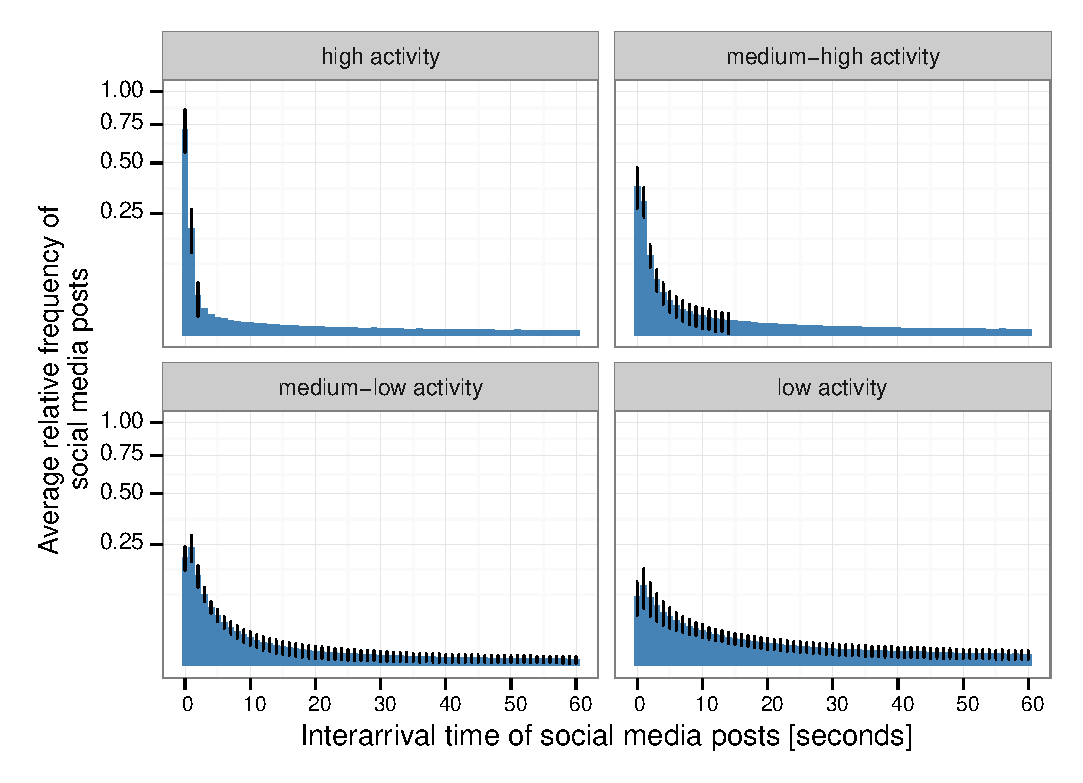
\includegraphics[width=\textwidth]{figures/high-activity/fig4}
  \caption[Average histograms of activity levels]{Average histograms of the high
      activity, medium-high activity, medium-low activity and low activity
      clusters in our dataset (from left to right and top to bottom). All
      histograms include standard deviation bars and were cut-off at 60 second
      length for better visibility.
      % \inote{change labels of x and y axis}
    }\label{fig:hi:avg-hist}
\end{figure}

Figure~\ref{fig:hi:avg-hist} shows the average histograms for events that belong
to the high activity, medium-high activity, medium-low activity and low-activity
clusters (displayed from left to right and top to bottom). 
%
All histograms show a quick decay in average relative frequency (resembling a
distribution from the exponential family). 
%
In particular, the high-activity group concentrates most of its activity in the
shortest inter-arrival rate, with lower activity groups mostly concentrating
their activity in the second bin with slower decay. 
%
Figure~\ref{fig:hi:scatter} further characterizes the differences in behavior of
the high and low-activity groups, showing that high-activity events concentrate
on average $70\%$ of their activity in the smallest bin ($0$ sec.), against
$8\%$ for low-activity events. 
%
In addition, Figure~\ref{fig:hi:cdf} (left) shows the cumulative distribution
function (CDF) for each group of events, and Figure~\ref{fig:hi:cdf} (right)
shows $\log{(1 - \mathrm{CDF})}$. 
%
Visual inspection shows a clear difference in how inter-arrival rates are
distributed within each group, however, these figures do not indicate a
power-law distribution nor exponential distribution.%%

\begin{figure}[!htb]
  \centering
    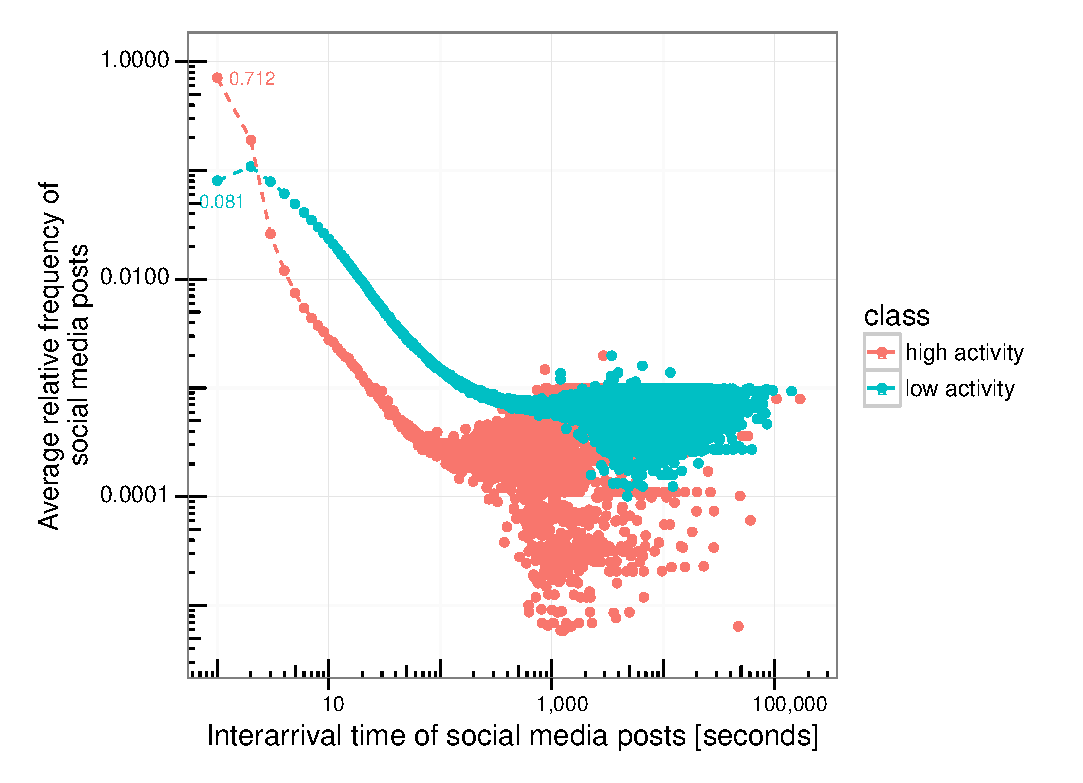
\includegraphics[width=\textwidth]{figures/high-activity/fig5}
  \caption[Relative frequencies of inter-arrival times]{Scatter plots of the
average relative frequencies of inter-arrival times for the high-activity and
low-activity clusters of events (i.e., scatter plots of the histograms in
Figure~\ref{fig:hi:avg-hist} in log-log scale). $y$-axis represents the average
relative frequency of social media messages and $x$-axis the inter-arrival time.}
\label{fig:hi:scatter}
\end{figure}

\begin{figure}
  \centering
  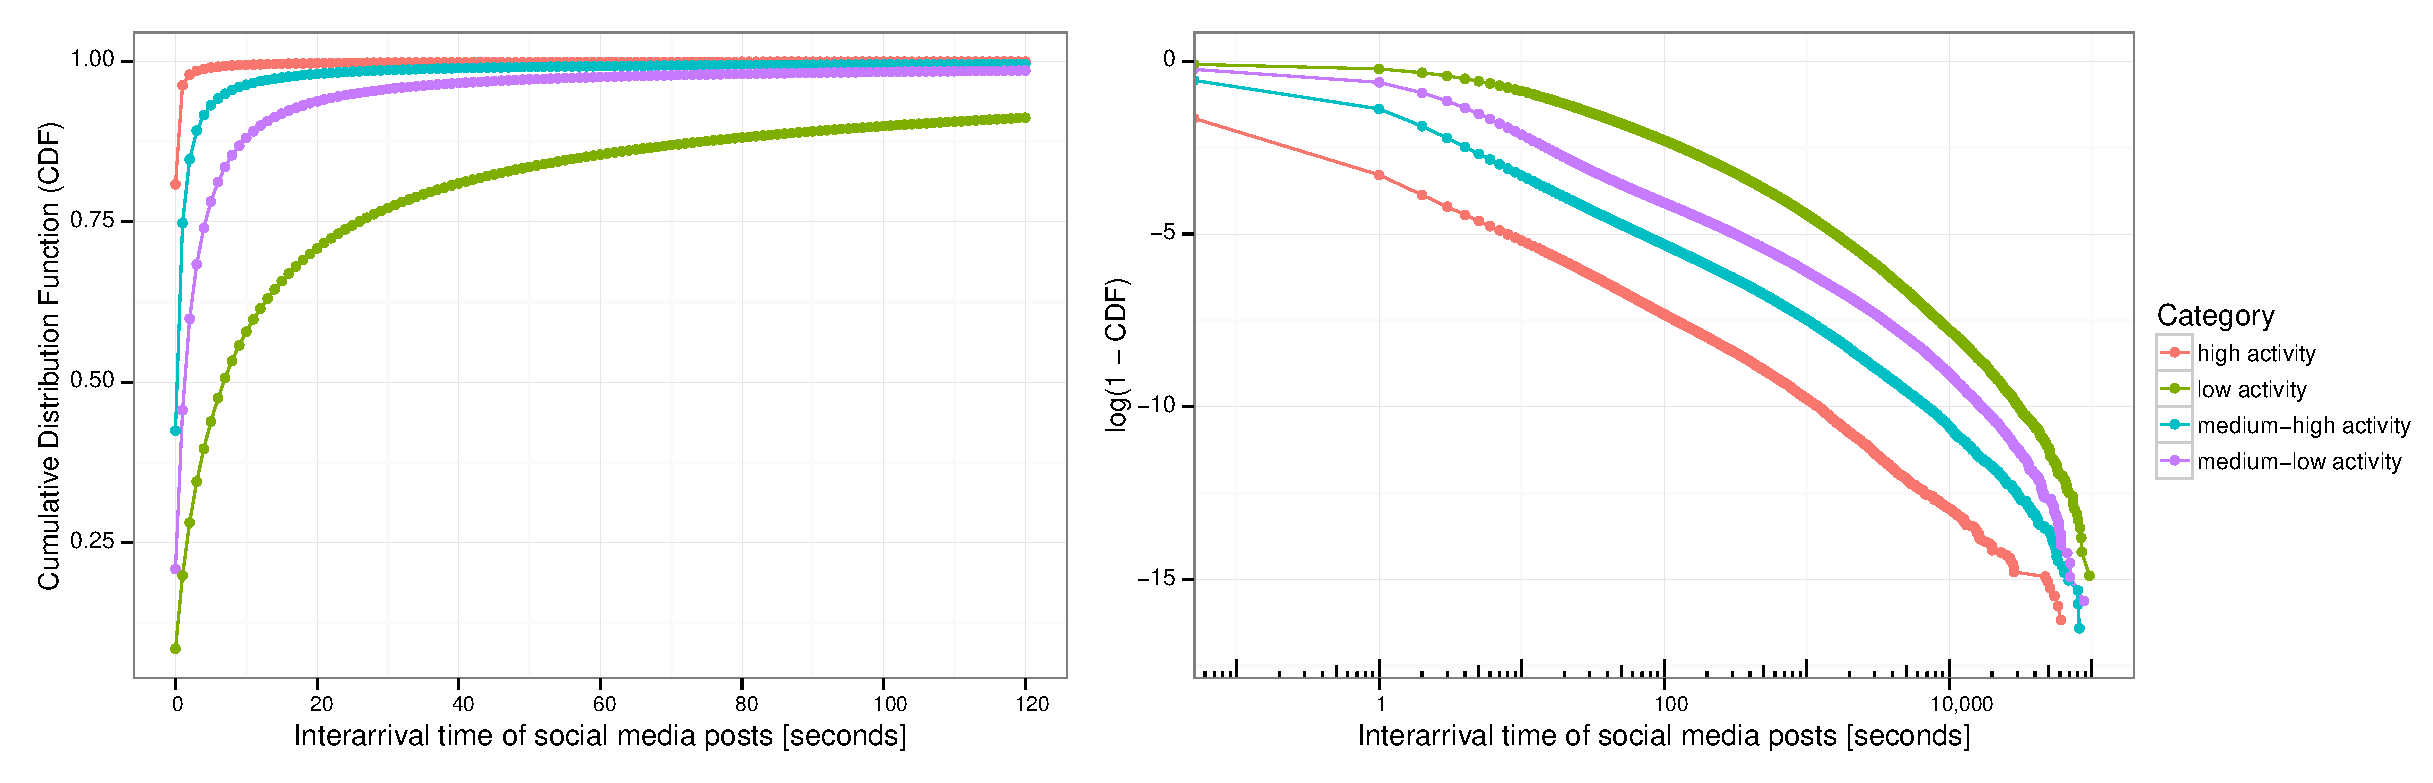
\includegraphics[width=\textwidth]{figures/high-activity/fig6_log}
  \caption[Cumulative Distribution Functions of activity levels]{{(Left) Average
cumulative distribution function (CDF) for the high activity, medium-high
activity, medium-low activity and low activity clusters in our dataset. (Right)
$\log{(1 - \mathrm{CDF})}$ for the same clusters. 
      % \inote{change labels of x and y axis}
    }}\label{fig:hi:cdf} %% fig6_long_inf_omitted.pdf
\end{figure}



Further analysis of the high-activity events shows significant differences to
other events, in the following aspects: 
%
(i) how the information about these events is propagated, 
%
(ii) the characteristics of the conversations that they generate, and 
%
(iii) how focused users are on the news topic. 

\subsection{Information Forwarding Characteristics}
\label{subsec:info_forwarding}

We found that high-activity events possess more information forwarding
characteristics than other events. 
%
We present four features which support this argument. 
%
The features, their description and their values are listed in
Table~\ref{tab:information_forwarding}.

The \texttt{retweet\_count} is generally higher for high-activity events.
%
This feature is the fraction of retweets present in the event, log-normalized by
the total amount of tweets in the event. 
%
A higher value suggests that people have a greater tendency to spread the
occurrence of these events, and forward this information to their followers. 

The \texttt{tweets\_retweeted} is lower for high-activity events than for the
rest. 
%
This feature is the number of tweets which have been retweeted, log-normalized
by the total number of tweets in the event. 
%
This suggests that the high amount of retweets for the high-activity events
actually originates from fewer tweets. This suggests that fewer tweets become
popular and are retweeted several times.

The \texttt{retweets\_most\_retweeted} is the total number of retweets of the
tweet that has been retweeted the most. 
%
This number is much higher for high-activity events than for low-activity
events, suggesting that the most popular tweet indeed becomes very popular when
the event is of high-impact.

\begin{table}
  \centering
  {\small
    \begin{tabular}{llll}
      \toprule
      Feature Name &  \multicolumn{1}{l}{Description} & high-activity, others& Hypothesis, $p$-value\\
      \midrule
      \texttt{retweet\_count} & \pbox{20cm}{$\log($total retweet count \\in the event divided by total\\ tweets in the event$)$} & $2.205, 1.473$ & $1$, $p = 0$ \\
      \midrule
      \texttt{tweets\_retweeted} & \pbox{20cm}{$\log($number of tweets \\retweeted divided by\\ total tweets in the event$)$} & $-1.091, -0.964$ & $1$, $p = 2.7\times10^{-5}$ \\
      \midrule
      \texttt{retweets\_most\_retweeted} & \pbox{20cm}{number of tweets of the most \\retweeted tweet} & $284.491, 40.261$ & $1$, $p = 0$ \\
      \bottomrule
    \end{tabular}
  }
  \caption[Information forwarding characteristics of events]{Features which characterize the information forwarding aspect of an event.
  In general, high-activity events tend to have higher values for information forwarding 
  features than other events.}
  \label{tab:information_forwarding}
\end{table}

%%

In summary, high-activity events have a higher fraction of {\em retweets} (or
shares) relative to their overall message volume. 
%
On average, a tweet from a high-activity event is retweeted 2.36 times more than
a tweet from a low activity event. 
%
The most retweeted message in high-activity events is retweeted 7 times more
than the most retweeted message in a medium or low activity event. 
%
We find that a small set of initial social media posts are propagated quickly
and extensively through the network without any rephrasing by the user (just
plain forwarding). 
%
Intuitively, this seems justified given general topic urgency of high-activity
events. 
%
Events that are not high-activity did not exhibit these characteristics.

% %%


\subsection{Conversational Characteristics}
\label{subsec:conversational}

We found that high-activity events in general tend to generate more conversation
between users than the events in other categories. 
%
We observe this behavior through several features. 
%
Refer to Table~\ref{tab:conversational}.

\begin{table}
  \centering
  {\small
    \begin{tabular}{llll}
      \toprule
      Feature Name &  \multicolumn{1}{l}{Description} & high-activity, others & Hypothesis, $p$-value\\
      \midrule
      \texttt{replies} & \pbox{20cm}{$\log($total replies divided by total tweets$)$} & $-1.4016, -1.6474$ & $1$, $p = 10^{-4}$ \\
      \midrule
      \texttt{norm\_replies} & \pbox{20cm}{$\log($number of replies divided by\\ total number of unique users$)$} & $-1.5796, -1.9294$ & $1$, $p = 6.7\times10^{-4}$ \\
      \midrule
      \texttt{tweets\_replied} & \pbox{20cm}{$\log($number of tweets which generated\\ replies divided by total tweets$)$} & $-1.7784, -2.0668$ & $1$, $p = 0.001$ \\
      \midrule
      \texttt{uniq\_users\_replied} & \pbox{20cm}{$\log($unique users who have written\\ a reply divided by total tweets$)$} & $-1.7524, -2.0352$ & $1$, $p = 0.001$ \\
      \bottomrule
    \end{tabular}
  } \caption[Conversational features of events]{Features which characterize the
  conversational aspect of high-activity and remaining events. We argue that
  high-activity events tend to invoke more conversation among users than their
  counterparts.}
  \label{tab:conversational}
\end{table}

The features \texttt{replies} and \texttt{norm\_replies} both count the number
of replies, but have been normalized slightly differently. 
%
Both have a higher value for high-activity events suggesting that high-activity
events in general tend to spark more conversation between the users. 
%
The \texttt{tweets\_replied} feature counts the number of tweets which have
generated replies (it has been log-normalized by the total number of tweets in
the event). 
%
This is also higher for high-activity indicating that such events on average
have more tweets which invoke a reply from people. 
%
The \texttt{uniq\_users\_replied} feature counts the number of unique users who
have participated in an conversation. 
%
Again, this number is found to be higher for high-activity events than for
others suggesting that more users tend to engage in a conversation about these
events. 
%
All these features collectively suggest that high-activity events tend to have a
\emph{conversational characteristic} associated with them.

%%

In summary, high-activity events tend to spark more conversation between users,
33.4\% more than other events. 
%
This is reflected in the number of {\em replies} to social media posts. 
%
The number of different users that engage with high-activity events is 32.7\%
higher than in events that are not high-activity. 



\subsection{Topical Focus Characteristics}
\label{subsec:topical_focus}


We find that high-activity events have a lot more focus in terms of the topical
content than the remaining events. 
%
This possibly suggests that when a news item is sensational, people seldom
deviate from the topic of the news to other things. 

We used four features listed in Table~\ref{tab:topical_focus} to study the topic
focus characteristics of high-impact events.

\begin{table}
  \centering
  {\small
    \begin{tabular}{llll}
      \toprule
      Feature Name &  \multicolumn{1}{l}{Description} & high-activity, others & Hypothesis, $p$-value\\
      \midrule
      \texttt{uniq\_words} & \pbox{20cm}{$\log($total unique words \\divided by total tweets$)$} & $-0.1982, 0.1651$ & $1$, $p = 0$ \\
      \midrule
      \texttt{uniq\_chars} & \pbox{20cm}{$\log($total unique characters \\divided by total tweets$)$} & $2.0009, 2.0456$ & $1$, $p = 0$ \\
      \midrule
      \texttt{uniq\_hashtags} & \pbox{20cm}{$\log($number of unique hashtags\\ divided by total tweets$)$} & $-1.1126, 0.8761$ & $1$, $p = 0$ \\
      \midrule
      \texttt{uniq\_urls} & \pbox{20cm}{$\log($number of unique urls \\divided by total tweets$)$} & $-0.7194, -0.4951$ & $1$, $p = 0$ \\
      \bottomrule
    \end{tabular}
  } \caption[Topical focus features of events]{Features that were used to study
  the topical focus characteristics of high-activity events.}
  \label{tab:topical_focus}
\end{table}

The number of unique words (\texttt{uniq\_words}) and characters
(\texttt{uniq\_chars}) for high-activity events is lower than the remaining
events suggesting that the information content for high-activity events is more
focused than for the remaining events (as they do not need a diverse
vocabulary). 
%
Hashtags on Twitter are a sequence of characters that follow the \# symbol.
%
Conventionally, their purpose is to indicate the topic of the tweet. 
%
Again, this number (\texttt{uniq\_hashtags}, log-normalized by the total number
of tweets) is lower for the high-activity events than for the remaining events.
%
The number of unique URLs (\texttt{uniq\_urls}, which can be taken to interpret
similar semantics as the hashtags) is also lower for high-activity events than
for the rest. 


%%

Summarizing, posts about high-activity events are much more topic focused than
in other events. 
%
The vocabulary of unique words as well as {\em hashtags} used in high-activity
events is much more narrow than for other events. 
%
Medium and low activity events have over 7 times more unique hashtags than
high-activity events. 
%
This is intuitive, given that if a news item is sensational, people will seldom
deviate from the main conversation topic.

%%

\subsection{Predicting the Activity of Events}

In a real-world scenario, in order to predict if an early breaking news story
will have a considerable impact in the social network, we will not have enough
data to create its activity-based model, i.e., we will not yet know the
distribution of the speed at which the social media posts will arrive for the
event. 
%
For instance, an event can start slowly and later produce an explosive reaction,
or start explosively and decay quickly to an overall slower message arrival
rate. 
%
Still, reliable early prediction of very high-activity news is important in many
aspects, from decisions of mass media information coverage, to natural disaster
management, brand and political image monitoring, and so on.

%%

For the task of early prediction of high-activity events we use features that
are independent of our activity-based model such as the retweets, the sentiment
of the posts about the event, etc. These features are computed on the early 5\%
of messages about the event.
%
A list of all the features used for classification is shown in Table
\ref{tab:feats}.
%
The results are an average from a 5-fold cross validation with randomly selected
60\% training, 20\% validation and 20\% test splits.
%
The classification was carried using logistic regression provided by the Weka
package.
%
The high-activity events are identified with a precision of 82\% using only the
earliest 5\% of the data of each event (Table~\ref{tab:classification_results}).
%
Additionally, we were able to identify with high accuracy a considerable
percentage of all high-activity events ($\approx 46\%$) at an early stage, with
very few false positives (Table~\ref{tab:classification_results}
and~\ref{tab:confusion_matrix}).

\begin{table}
  %\begin{adjustwidth}{-10mm}{-10mm}
  \centering
  {\small
    \begin{tabularx}{\textwidth}{lcccc|cccc}
      \toprule
      & \multicolumn{4}{c}{\textbf{Early 5\% Tweets}} & \multicolumn{4}{c}{\textbf{All Tweets}} \\
      \midrule
      & FP-Rate & Precision & Recall & ROC-area & FP-Rate & Precision & Recall & ROC-area \\
      % \midrule
      high-activity & 0.009 & 0.819 & 0.455 & 0.900 & 0.01 & 0.830 & 0.540 & 0.945 \\
      non-high-activity & 0.545 & 0.954 & 0.991 & 0.900 &  0.460 & 0.960 & 0.990 & 0.945 \\
      \bottomrule
    \end{tabularx}
  }
  \caption{{Classification results of high-activity events.}}
  \label{tab:classification_results}
  %\end{adjustwidth}
%                                                                                                                                448,1         93%
\end{table}

\begin{table}
  \centering
  % {\scriptsize
  \begin{tabularx}{\textwidth}{lcc|cc}
    \toprule
    \multirow{2}{*}{ }& \multicolumn{2}{c}{\textbf{Early 5\% Tweets}} & \multicolumn{2}{c}{\textbf{All Tweets}} \\
    \midrule
    % \cmidrule{2-5} \cline{2-5}
    & high-activity & non-high-activity & high-activity & non-high-activity \\
    % \midrule
    high-activity & $194$ & $232$ & $230$ & $196$\\
    non-high-activity & $43$ & 4,765 & 47 & 4,761 \\
    \bottomrule
  \end{tabularx}
  % }
  \caption{{Confusion matrix for high-activity events prediction.}}
  \label{tab:confusion_matrix}
\end{table}



The precision using only the early tweets is almost as good as using all tweets
in the event (0.819 to 0.830). 
%
This suggests that the social network somehow acts as a natural filter in
separating out the high-activity events fairly early on.  
%
The recall goes from 0.455 to 0.540. 
%
This indicates that there are some high-activity events which require more data
in order to determine what kind of activity they will produce, or events for
which activity occurs due to random conditions. 



{\footnotesize
  \begin{longtable}{l|l|l}

    \hline \textbf{Feature Name} & \textbf{Normalized By} &
    \textbf{Normalization
      Method} \\
    \hline
    \endfirsthead
    \multicolumn{3}{l}%
    {\tablename\ \thetable\ -- \textit{Continued from previous page}} \\
    \hline \textbf{Feature Name} & \textbf{Normalized By} &
    \textbf{Normalization
      Method} \\
    \hline
    \endhead
    \hline \multicolumn{3}{l}{\textit{Continued on next page}} \\
    \endfoot
    \hline
    \endlastfoot


    \texttt{component\_size}	&	 None	&	  \\
    \texttt{total\_seconds}	&	 \texttt{total\_tweets}	& $\log(x) - \log(y)$ \\
    \texttt{total\_tweets}	&	 None	&	  \\
    \texttt{total\_retweets}	&	 \texttt{total\_tweets}	&	 $\log(x) - \log(y)$ \\
    \texttt{total\_tweets\_retweeted}	&	 \texttt{total\_tweets}	&	 $\log(x) - \log(y)$ \\
    \texttt{retweets\_most\_retweeted}	&	 \texttt{total\_retweets}	&	 $\log(x) - \log(y)$ \\
    \texttt{total\_mentions}	&	 \texttt{total\_tweets}	&	 $\log(x) - \log(y)$ \\
    \texttt{total\_unique\_mentions} &
    \texttt{total\_mentions}	&	 $\log(x) - \log(y)$ \\
    \texttt{total\_tweets\_with\_mention}	&	 \texttt{total\_tweets}	&	 $\log(x) - \log(y)$ \\
    \texttt{total\_tweets\_with\_mostfrequent\_mention}	&	 \texttt{total\_tweets\_with\_mention}	&	 $\log(x) - \log(y)$ \\
    \texttt{total\_hashtags}	&	 \texttt{total\_tweets}	&	 $\log(x) - \log(y)$ \\
    \texttt{total\_unique\_hashtags}	&	 \texttt{total\_hashtags}	&	 $\log(x) - \log(y)$ \\
    \texttt{total\_tweets\_with\_hashtag}	&	 \texttt{total\_tweets}	&	 $\log(x) - \log(y)$ \\
    \texttt{total\_tweets\_with\_mostfrequent\_hashtag}	&	 \texttt{total\_tweets\_with\_hashtag}	&	 $\log(x) - \log(y)$ \\
    \texttt{total\_urls}	&	 \texttt{total\_tweets}	&	 $\log(x) - \log(y)$ \\
    \texttt{total\_unique\_urls}	&	 \texttt{total\_urls}	&	 $\log(x) - \log(y)$ \\
    \texttt{total\_tweets\_with\_url}	&	 \texttt{total\_tweets}	&	 $\log(x) - \log(y)$ \\
    \texttt{total\_tweets\_with\_mostfrequent\_url}	&	 \texttt{total\_tweets\_with\_url}	&	 $\log(x) - \log(y)$ \\
    \texttt{total\_unique\_verified\_users}	&	 \texttt{total\_verified\_users}	&	 $\log(x) - \log(y)$ \\
    \texttt{total\_verified\_users}	&	 \texttt{total\_tweets}	&	 $\log(x) - \log(y)$ \\
    \texttt{total\_unique\_users}	&	 \texttt{total\_tweets}	&	 $\log(x) - \log(y)$ \\
    \texttt{total\_replies} & \texttt{total\_unique\_users} &
    $\log(x) - \log(y)$ \\
    \texttt{total\_tweets\_first\_replied} & \texttt{total\_tweets} &
    $\log(x) - \log(y)$ \\
    \texttt{total\_unique\_users\_replied} &
    \texttt{total\_unique\_users} &
    $\log(x) - \log(y)$ \\
    \texttt{total\_tweets\_replied}	&	 \texttt{total\_tweets}	&	 $\log(x) - \log(y)$ \\
    \texttt{total\_words}	&	 \texttt{total\_tweets}	&	 $\log(x) - \log(y)$ \\
    \texttt{total\_unique\_words}	&	 \texttt{total\_words}	&	 $\log(x) - \log(y)$ \\
    \texttt{total\_characters}	&	 \texttt{total\_tweets}	&	 $\log(x) - \log(y)$ \\
    \texttt{total\_rt\_count}	&	 \texttt{total\_tweets}	&	 $\log(x) - \log(y)$ \\
    \texttt{total\_fav\_count}	&	 \texttt{total\_tweets}	&	 $\log(x) - \log(y)$ \\
    \texttt{total\_positive\_sentiment}	& \texttt{total\_tweets}	&	 $x / y$ \\
    \texttt{total\_negative\_sentiment}	&	 \texttt{total\_tweets}	&	 $x / y$ \\
    \hline

    \caption[Features used for classification of activity]{List of
        features used for characterization and classification. The
        ``Normalization Method'' column corresponds to the method used to
        normalize the value of the first column using the value of the second
        column. For example, the total number of retweets was normalized
        dividing it by the total number of tweets, and then taking the
        logarithm. Zero values were replaced by $10^{-8}$.}
    \label{tab:feats}
  \end{longtable}}

